\begin{minipage}{9cm}
\begin{enumerate}
\item Adam a réalisé le programme ci-contre à l’aide du logiciel Scratch.
\begin{enumerate}
	\item Montrer que si le nombre de départ est 3, le résultat est égal à 9.
	\item Quel est le résultat donné par le programme si le nombre de départ est 2,4 ?
	\item Soit $x$ le nombre de départ. Montrer que le programme d’Adam retourne le nombre $2x^2 - x - 6$.
\end{enumerate}
\end{enumerate}
\end{minipage}
\hfill
\begin{minipage}{9cm}
\begin{scratch}[scale=0.75,print]
		\blockinit{quand \greenflag est cliqué}
		\blocksensing{demander \ovalnum{Choisis un nombre} et attendre}
		\blockvariable{mettre \selectmenu{nombre départ} à \ovalsensing{réponse}}
		\blockvariable{mettre \selectmenu{valeur 1} à \ovaloperator{\ovalvariable{2} * \ovalvariable{nombre départ}}}
		\blockvariable{mettre \selectmenu{valeur 2} à \ovaloperator{\ovalvariable{valeur 1} + \ovalvariable{3}}}		
		\blockvariable{mettre \selectmenu{valeur 3} à \ovaloperator{\ovalvariable{nombre départ} - \ovalvariable{2}}}				\blockvariable{mettre \selectmenu{résultat} à \ovaloperator{\ovalvariable{valeur 2} * \ovalvariable{valeur 3}}}	        \blocklook{dire \ovaloperator{regrouper \ovalnum{Le résultat du programme est } et \ovalvariable{résultat}}}	\end{scratch}
\end{minipage}

\begin{enumerate}
	\setcounter{enumi}{2}
	\item Pauline propose le programme de calcul suivant.
	\begin{center}
	\begin{tabular}{|c|}
	\hline
	Choisis un nombre\\
	Élève-le au carré\\
	Soustrais 3.\\
	Multiplie par 2.\\
	Soustrais le nombre de départ.\\ 
	\hline 
	\end{tabular} 
	\end{center}
	\begin{enumerate}
		\item Montrer que si le nombre de départ est 3, le résultat obtenu est égal à 9.
		\item Quel est le résultat donné par le programme si le nombre de départ est $\dfrac{7}{3}$ ?
	\end{enumerate}
	\item Montrer que, pour un même nombre de départ, les programmes de calcul d’Adam et
Pauline donnent le même résultat.
	\item Déterminer le ou les nombres de départ possibles pour que les résultats des programmes
de calcul soient nuls. Justifier.
	\item Adam souhaite automatiser les calculs de son programme pour les entiers naturels. Il
utilise un tableur dont la copie d’écran est donnée ci-dessous.
Quelle formule doit-il saisir dans la case B2 pour qu'il puisse l’étirer vers le bas sur
l'ensemble de la colonne ?
\begin{center}
	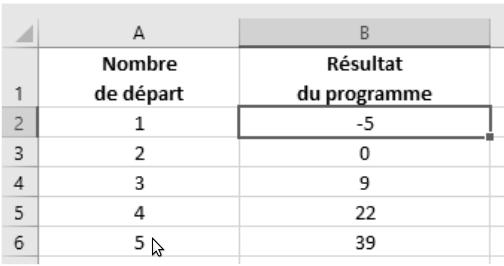
\includegraphics[width=.5\textwidth]{./images/2022-g2-ex4-img1.png}
\end{center}
\end{enumerate}
